\documentclass[]{article}

% Math packages
\usepackage[usenames]{color}
\usepackage{forest}
\usepackage{ifxetex,ifluatex,amsmath,amssymb,mathrsfs,amsthm,witharrows,mathtools}
\WithArrowsOptions{displaystyle}
\renewcommand{\qedsymbol}{$\blacksquare$} % end proofs with \blacksquare. Overwrites the defualts. 
\usepackage{cancel,bm}
\usepackage[thinc]{esdiff}

% tikz
\usepackage{tikz}
\newcommand\sqw{1}
\newcommand\squ[4][1]{\fill[#4] (#2*\sqw,#3*\sqw) rectangle +(#1*\sqw,#1*\sqw);}


% code 
\usepackage{listings}
\usepackage{xcolor}

\definecolor{codegreen}{rgb}{0,0.35,0}
\definecolor{codegray}{rgb}{0.5,0.5,0.5}
\definecolor{codenumber}{rgb}{0.1,0.3,0.5}
\definecolor{codeblue}{rgb}{0,0,0.5}
\definecolor{codered}{rgb}{0.5,0.03,0.02}
\definecolor{codegray}{rgb}{0.9,0.9,0.9}

\lstdefinestyle{pythonstylesheet}{
	language=Python,
	emphstyle=\color{deepred},
	backgroundcolor=\color{codegray},
	keywordstyle=\color{deepblue}\bfseries\itshape,
	numberstyle=\scriptsize\color{codenumber},
	basicstyle=\ttfamily\footnotesize,
	breakatwhitespace=false, 
	breaklines=true, 
	captionpos=b, 
	keepspaces=true, 
	numbers=left, 
	numbersep=5pt, 
	showspaces=false,                
	showstringspaces=false,
	showtabs=false, 
	tabsize=2, 
	morekeywords={object,type,isinstance,copy,deepcopy,zip,enumerate,reversed,list,set,len,dict,tuple,range,xrange,append,execfile,real,imag,reduce,str,repr},              % Add keywords here
	keywordstyle=\color{codeblue},
	emph={__init__,__add__,__mul__,__div__,__sub__,__call__,__getitem__,__setitem__,__eq__,__ne__,__nonzero__,__rmul__,__radd__,__repr__,__str__,__get__,__truediv__,__pow__,__name__,__future__,__all__,as,assert,nonlocal,with,yield,self,True,False,None,AssertionError,ValueError},          % Custom highlighting
	emphstyle=\color{codered},
	stringstyle=\color{codegreen},
	showstringspaces=false,
	abovecaptionskip=0pt,belowcaptionskip =0pt,
	framextopmargin=-\topsep, 
}
\newcommand\pythonstyle{\lstset{pythonstylesheet}}
\newcommand\pyl[1]     {{\lstinline!#1!}}
\lstset{style=pythonstylesheet}

\usepackage[style=1,skipbelow=\topskip,skipabove=\topskip,framemethod=TikZ]{mdframed}
\definecolor{bggray}{rgb}{0.85, 0.85, 0.85}
\mdfsetup{leftmargin=0pt,rightmargin=0pt,backgroundcolor=codegray,middlelinewidth=0.5pt,skipabove=4pt,skipbelow=0pt,middlelinecolor=black,roundcorner=5}
\BeforeBeginEnvironment{lstlisting}{\begin{mdframed}\vspace{-0.4em}}
\AfterEndEnvironment{lstlisting}{\vspace{-0.8em}\end{mdframed}}
	
% Deisgn
\usepackage[labelfont=bf]{caption}
\usepackage[margin=0.6in]{geometry}
\usepackage{multicol}
\usepackage[skip=4pt, indent=0pt]{parskip}
\usepackage[normalem]{ulem}
\forestset{default}
\renewcommand\labelitemi{$\bullet$}
\usepackage{titlesec}
\titleformat{\section}[block]
	{\fontsize{15}{15}}
	{\sen \dotfill \, \!\!\! \thesection \,\! \dotfill \she}
	{0em}
	{\MakeUppercase}
\usepackage{graphicx}
\graphicspath{ {./} }

% Hebrew initialzing
\usepackage[bidi=basic]{babel}
\babelprovide[main, import]{hebrew}
\babelfont{rm}{David CLM}
\babelfont{sf}{David CLM}
\babelfont{tt}{Monaspace Argon}
\usepackage[shortlabels]{enumitem}
\newlist{hebenum}{enumerate}{1}

% Language Shortcuts
\newcommand\en[1] {\selectlanguage{english}#1\selectlanguage{hebrew}}
\newcommand\sen   {\selectlanguage{english}}
\newcommand\she   {\selectlanguage{hebrew}}
\newcommand\del   {$ \!\! $}
\newcommand\ttt[1]{\en{\small\texttt{#1}\normalsize}}

\newcommand\npage {\vfil {\hfil \textbf{\textit{המשך בעמוד הבא}}} \hfil \vfil \pagebreak}
\newcommand\ndoc  {\dotfill \\ \vfil {\begin{center} {\textbf{\textit{שחר פרץ, 2024}} \\ \scriptsize \textit{נוצר באמצעות תוכנה חופשית בלבד}} \end{center}} \vfil	}

\newcommand{\rn}[1]{
	\textup{\uppercase\expandafter{\romannumeral#1}}
}

\makeatletter
\newcommand{\skipitems}[1]{
	\addtocounter{\@enumctr}{#1}
}
\makeatother

%! ~~~ Math shortcuts ~~~

% Letters shortcuts
\newcommand\N     {\mathbb{N}}
\newcommand\Z     {\mathbb{Z}}
\newcommand\R     {\mathbb{R}}
\newcommand\Q     {\mathbb{Q}}
\newcommand\C     {\mathbb{C}}

\newcommand\ml    {\ell}
\newcommand\mj    {\jmath}
\newcommand\mi    {\imath}

\newcommand\powerset {\mathcal{P}}
\newcommand\ps    {\mathcal{P}}
\newcommand\pc    {\mathcal{P}}
\newcommand\ac    {\mathcal{A}}
\newcommand\bc    {\mathcal{B}}
\newcommand\cc    {\mathcal{C}}
\newcommand\dc    {\mathcal{D}}
\newcommand\ec    {\mathcal{E}}
\newcommand\fc    {\mathcal{F}}
\newcommand\nc    {\mathcal{N}}
\newcommand\sca   {\mathcal{S}} % \sc is already definded
\newcommand\rca   {\mathcal{R}} % \rc is already definded

\newcommand\Si    {\Sigma}

% Logic & sets shorcuts
\newcommand\siff  {\longleftrightarrow}
\newcommand\ssiff {\leftrightarrow}
\newcommand\so    {\longrightarrow}
\newcommand\sso   {\rightarrow}

\newcommand\epsi  {\epsilon}
\newcommand\vepsi {\varepsilon}
\newcommand\vphi  {\varphi}
\newcommand\Neven {\N_{\mathrm{even}}}
\newcommand\Nodd  {\N_{\mathrm{odd }}}
\newcommand\Zeven {\Z_{\mathrm{even}}}
\newcommand\Zodd  {\Z_{\mathrm{odd }}}
\newcommand\Np    {\N_+}

% Text Shortcuts
\newcommand\open  {\big(}
\newcommand\qopen {\quad\big(}
\newcommand\close {\big)}
\newcommand\also  {\text{, }}
\newcommand\defi  {\text{ definition}}
\newcommand\defis {\text{ definitions}}
\newcommand\given {\text{given }}
\newcommand\case  {\text{if }}
\newcommand\syx   {\text{ syntax}}
\newcommand\rle   {\text{ rule}}
\newcommand\other {\text{else}}
\newcommand\set   {\ell et \text{ }}
\newcommand\ans   {\mathit{Ans.}}

% Set theory shortcuts
\newcommand\ra    {\rangle}
\newcommand\la    {\langle}

\newcommand\oto   {\leftarrow}

\newcommand\QED   {\quad\quad\mathscr{Q.E.D.}\;\;\blacksquare}
\newcommand\QEF   {\quad\quad\mathscr{Q.E.F.}}
\newcommand\eQED  {\mathscr{Q.E.D.}\;\;\blacksquare}
\newcommand\eQEF  {\mathscr{Q.E.F.}}
\newcommand\jQED  {\mathscr{Q.E.D.}}

\newcommand\dom   {\text{dom}}
\newcommand\Img   {\text{Im}}
\newcommand\range {\text{range}}

\newcommand\trio  {\triangle}

\newcommand\rc    {\right\rceil}
\newcommand\lc    {\left\lceil}
\newcommand\rf    {\right\rfloor}
\newcommand\lf    {\left\lfloor}

\newcommand\lex   {<_{lex}}

\newcommand\az    {\aleph_0}
\newcommand\uaz   {^{\aleph_0}}
\newcommand\al    {\aleph}
\newcommand\ual   {^\aleph}
\newcommand\taz   {2^{\aleph_0}}
\newcommand\utaz  { ^{\left (2^{\aleph_0} \right )}}
\newcommand\tal   {2^{\aleph}}
\newcommand\utal  { ^{\left (2^{\aleph} \right )}}
\newcommand\ttaz  {2^{\left (2^{\aleph_0}\right )}}

\newcommand\n     {$n$־יה\ }

% Math A&B shortcuts
\newcommand\logn  {\log n}
\newcommand\cosx  {\cos x}
\newcommand\cost  {\cos \theta}
\newcommand\sex   {\sec x}        % NICE
\newcommand\cotx  {\cot x}
\newcommand\sinx  {\sin x}
\newcommand\sint  {\sin \theta}
\newcommand\tanx  {\tan x}
\newcommand\tant  {\tan \theta}

\newcommand\coshx  {\cosh x}
\newcommand\sinhx  {\sinh x}
\newcommand\tanhx  {\tanh x}

\newcommand\arccosh {\mathrm{arccosh}\,}
\newcommand\arcsinh {\mathrm{arcsinh}\, }
\newcommand\arctanh {\mathrm{arctanh}\, }

\newcommand\dx    {\,\mathrm{d}x}
\newcommand\df    {\mathrm{d}f}
\newcommand\dfdx  {\diff{f}{x}}
\newcommand\dit   {\limhz \frac{f(x + h) - f(x)}{h}}

\newcommand\nt[1] {\frac{#1}{#1}}

\newcommand\seq   {\overset{!}{=}}
\newcommand\sle   {\overset{!}{\le}}
\newcommand\sge   {\overset{!}{\ge}}
\newcommand\sll   {\overset{!}{<}}
\newcommand\sgg   {\overset{!}{>}}

\newcommand\h     {\hat}
\newcommand\ve    {\vec}
\newcommand\lv    {\overrightarrow}
\newcommand\ol    {\overline}

\newcommand\mlcm  {\mathrm{lcm}}

\newcommand\limz  {\lim_{x \to 0}}
\newcommand\limhz {\lim_{h \to 0}}
\newcommand\limh  {\lim_{h \to 0}}
\newcommand\limxz {\lim_{x \to x_0}}
\newcommand\limi  {\lim_{x \to \infty}}
\newcommand\limni {\lim_{x \to - \infty}}
\newcommand\limpmi{\lim_{x \to \pm \infty}}

\newcommand\ta    {\theta}
\newcommand\ap    {\alpha}

\renewcommand\inf {\infty}
\newcommand  \ninf{-\inf}

% Combinatorics shortcuts
\newcommand\sumnk     {\sum_{k = 0}^{n}}
\newcommand\sumni     {\sum_{i = 0}^{n}}
\newcommand\sumnko    {\sum_{k = 1}^{n}}
\newcommand\sumnio    {\sum_{i = 1}^{n}}
\newcommand\sumai     {\sum_{i = 1}^{n} A_i}
\newcommand\nsum[2]   {\reflectbox{\displaystyle\sum_{\reflectbox{\scriptsize$#1$}}^{\reflectbox{\scriptsize$#2$}}}}

\newcommand\bink      {\binom{n}{k}}

\newcommand\cupain    {\bigcup_{i = 1}^{n} A_i}
\newcommand\cupai[1]  {\bigcup_{i = 1}^{#1} A_i}
\newcommand\cupiiai   {\bigcup_{i \in I} A_i}

\newcommand\xot       {x_{1, 2}}
\newcommand\ano       {a_{n - 1}}
\newcommand\ant       {a_{n - 2}}

% Other shortcuts
\newcommand\tl    {\tilde}
\newcommand\op    {^{-1}}
\newcommand\sof[1]    {\left | #1 \right |}
\newcommand\cl [1]    {\left ( #1 \right )}
\newcommand\csb[1]    {\left [ #1 \right ]}

\newcommand\bs    {\blacksquare}

%! ~~~ Document ~~~

\author{שחר פרץ}
\title{מבוא מורחב למדעי המחשב $\sim$ תרגיל בית מספר 1}

\begin{document}
	\maketitle
	\stepcounter{section} %%1
	\section{} %%2
	\subsection*{סעיף א'} פירוט והסבר השגיאות שהתקבלו: 
	\begin{enumerate}[1.]
		\item אם נריץ על טיפוס שאינו מחרוזת, נקבל את השגיאה: 
		\sen \begin{lstlisting}
Exception has occurred: AssertionError
exception: no description \end{lstlisting} \she				זאת מכיוון שהביטוי \ttt{ininstance(id\_num,str)} בעל ערך \ttt{False} בעבור \ttt{id\_num} מטיפוס שאינו \ttt{str}, על כן ה־keyword ``\ttt{assert}'' תקפיץ שגירה. 
				\item אם נריץ על מחרוזת באורך קצר מ־8, נקבל את השגיאה: 
			\sen \begin{lstlisting}
Exception has occurred: AssertionError
exception: no description \end{lstlisting} \she				זאת מכיוון שהביטוי \ttt{len(id\_num) == 8} בעל ערך \ttt{False} בעבור \ttt{id\_num} באורך שאינו $8$, על כן ה־keyword ``\ttt{assert}'' תקפיץ שגיאה. 
				\item אם צריץ על מחרוזת באורך 8 המכילה תווים שאינם ספרות, נקבל את השגיאה: 
			\sen \begin{lstlisting}
Exception has occurred: ValueError
invalid literal for int() with base 10: 'a'\end{lstlisting} \she
משום שבשורה \ttt{val = int(id\_num[i])} נעשה נסיון להמיר את התו במיקום ה־$i$ (ונעשה מעבר על כל המיקומים) ממחרוזת למספר, אך התו ``a'' לא מסמל שום מספר בבסיס 10 (ערך ברירת־המחדל של המתודה \ttt{int}). 
	\end{enumerate}
	\subsection*{סעיף ב'} אם נסיר את הפקודות המתחילות במילה \ttt{assert}, אז הפונקציה לא תבדוק יותר את תקינות הקלט, ותקיץ שגיאות אחרות שנובעות מאופן המימוש עצמו. לדוגמה, עבור טיפוסים שאינם מחרוזת נקבל (ככל הנראה, כתלות בקלט) \ttt{TypeError} כשנרצה לגשת לאינדקס של טיפוס שלא תומך בזאת, ועבור מחרוזות מתחת לאורך של $8$ תווים נקבל \ttt{IndexError} כשפייתון ינסה לגשת לאינדקס גבוהה מדי שלא קיים במחרוזת. 
	\subsection*{סעיף ג'} טבלת מעקב עבור \ttt{control\_digit("87654321")}: 
	\begin{center}
		\sen
		\begin{tabular}{|c|c|c|c|c|}
			\hline Iteration & \ttt{i} & \ttt{id\_num[i]} & \ttt{val} & \ttt{total} \\
			\hline 1 & 0 & "8" & 8 & 8 \\
			\hline 2 & 1 & "7" & 7 & 13 \\
			\hline 3 & 2 & "6" & 6 & 19 \\
			\hline 4 & 3 & "5" & 5 & 20 \\
			\hline 5 & 4 & "4" & 4 & 24 \\
			\hline 6 & 5 & "3" & 3 & 30 \\
			\hline 7 & 6 & "2" & 2 & 32 \\
			\hline 8 & 7 & "1" & 1 & 34 \\
			\hline 
		\end{tabular} \she
	\end{center}
	\pagebreak
	טבלת מעקב עבור \ttt{control\_digit("33455896")} (ת.ז. שלי): 
		
	\begin{center}
		\sen
		\begin{tabular}{|c|c|c|c|c|}
			\hline Iteration & \ttt{i} & \ttt{id\_num[i]} & \ttt{val} & \ttt{total} \\
			\hline 1 & 0 & "3" & 3 & 3 \\
			\hline 2 & 1 & "3" & 3 & 9 \\
			\hline 3 & 2 & "4" & 4 & 13 \\
			\hline 4 & 3 & "5" & 5 & 14 \\
			\hline 5 & 4 & "5" & 5 & 19 \\
			\hline 6 & 5 & "8" & 8 & 26 \\
			\hline 7 & 6 & "9" & 9 & 35 \\
			\hline 8 & 7 & "6" & 6 & 38 \\
			\hline 
		\end{tabular} \she
	\end{center}
	
\npage
\section{} %%3

\subsection*{סעיף א'} מדידות הזמן בעבור שני הפתרונות הראשונים: 
\sen \begin{center}
	\begin{tabular}{|c|c|c|c|}
		\hline input      & \ttt{zeros()}          & \ttt{zeros2()}         & output \\
		\hline $2^{100}$  & $2.297 \cdot 10^{-5}s$ & $2.211 \cdot 10^{-5}s$ & 6  \\
		\hline $2^{250}$  & $1.864 \cdot 10^{-5}s$ & $8.073 \cdot 10^{-6}$  & 11 \\
		\hline $2^{600}$  & $3.577 \cdot 10^{-5}s$ & $1.596 \cdot 10^{-5}s$ & 16 \\
		\hline $2^{1400}$ & $1.023 \cdot 10^{-4s}$ & $3.582 \cdot 10^{-5}s$ & 31 \\
		\hline
	\end{tabular}
\end{center} \she			נשים לב, שפרט עבור החישוב הראשון והשני (בהם משום מה המהירות קטנה עבור קלט גדול יותר), כמות הזמן תגדל כתלות בקלט. נתבונן בגרף המתאר את החישובים: 
	\begin{center}
	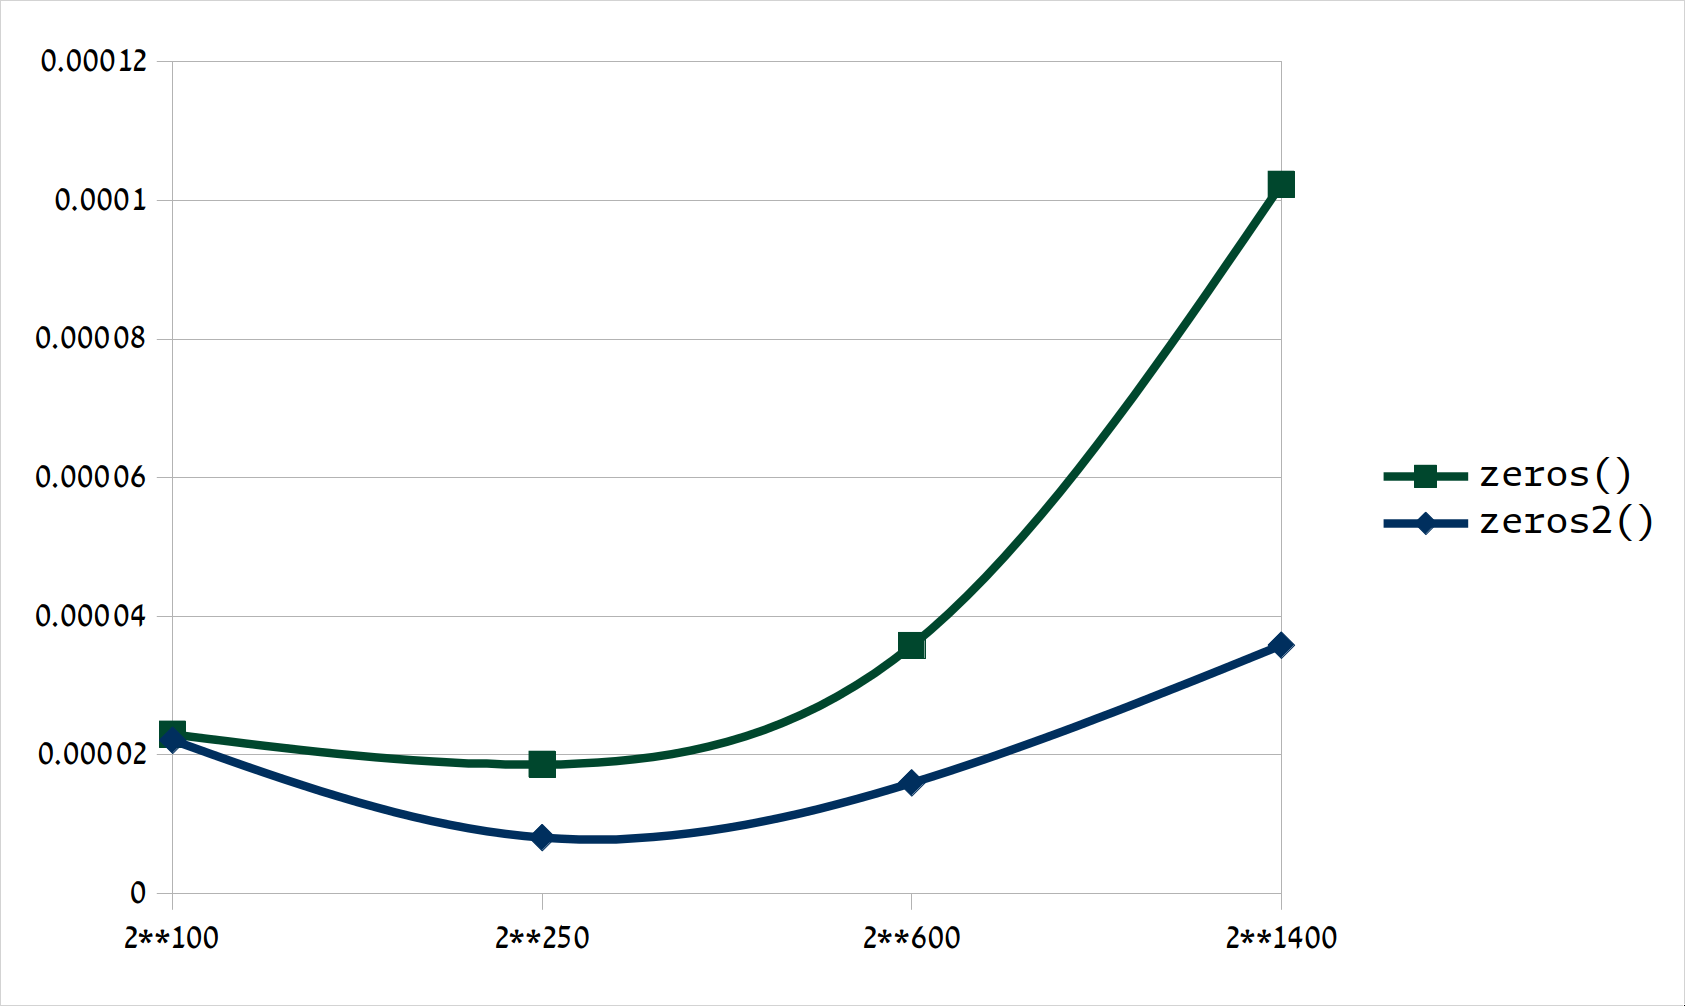
\includegraphics[scale=0.2]{Graph}
\end{center}			כלומר, עבור קלט שגדל באופן מעריכי, סיבוכיות הפונקציה \ttt{zeros()} תדמה להיות מעריכית, ו־\ttt{zeros2()} ליניארית (אם כי, בהתבוננות בקוד, נבין שאין זו ההתנהגות האמיתית בשאיפה לאינסוף). 
\subsection*{סעיף ב'} להלן התוצאות בעבור הפתרון השלישי: 
\sen \begin{center}
	\begin{tabular}{|c|c|c|}
		\hline input      & \ttt{zeros3()}         & output \\
		\hline $2^{100}$  & $1.404 \cdot 10^{-5}s$ & 6  \\
		\hline $2^{250}$  & $1.892 \cdot 10^{-6}s$ & 11 \\
		\hline $2^{600}$  & $2.301 \cdot 10^{-6}s$ & 16 \\
		\hline $2^{1400}$ & $3.56 \cdot 10^{-6s}$  & 31 \\
		\hline
	\end{tabular}
\end{center} \she			כלומר, הפונקציה תחזיר בקביעות פתרונות מהירים בערך פי $10$ מאלו של \ttt{zeros2()} (זה גם הגיוני שתהיה להם אותה התנהגות אסימפטוטית, כי הם ממומשים עם הגיון דומה) – כלומר, היא מהירה פי קבוע, אך לא אסימפטוטית, מ־\ttt{zeros2()}. 
\subsection*{סעיף ג'} לדוגמה, בעבור הקלטים $10^{100000} - 1, 10^{99999}$ (שניהם עם $999$ ספרות) נקבל: 
\begin{center} \sen \begin{tabular}{|c|c|c|c|c|}
	\hline input             & \ttt{zeros()} & \ttt{zeros2()} & \ttt{zeros3()} & output \\
	\hline $10^{100000} - 1$ & $2.5975s$ & $0.0325s$ & $0.0251s$ & 0  \\
	\hline $10^{99999}$      & $2.6043s$ & $0.0345s$ & $0.0237s$ & 99999 \\
	\hline
\end{tabular} \she \end{center}	נסיק, שהשינוי בזמן זניח, וייתכן שנגרם בגלל שגיאת מדידה. הסבר אפשרי לעליה מזערית בזמן במימושים של \ttt{zeros()} ו־\ttt{zeros2()}, הוא שייתכן ונגרם מהפעולה הנוספת של \ttt{cnt=cnt+1} במספרים עם יותר אפסים, זאת תחת ההנחה שהשינוי לא נגרם משגיאת מדידה (כנראה שלא כי התוצאות הורצו מספר פעמים). 
\subsection*{סעיף ד'} מסעיף (א), תוך הזנחת שאר הפעולות פרט ל־\ttt{cnt+=1} (מתוך הנחה שזה לא משפיע על סדר הגודל), ידוע שכמות הזמן שלוקח לחשב $\log_{10}(2^{1400})$ את השורה הזו, היא $3.58 \cdot 10^{-5}$ שניות. הלולאה שניתנה בסעיף הזה, תחזור על השורה הזו $2^{1000}$ פעמים, כלומר נחשב את היחס בין כמות הפעולות, ונמצא: 
\[ \frac{2^{1000}}{\log_{10}(2^{1400})} \cdot 3.58 \cdot 10^{-5} \approx 10^{294}s \]		(אך זהו רק חסם עליון, אם כי די הדוק בסדר הגודל). כאן, נוכל להבחין בהפרש הזמנים בין סיבוכיות לוגוריתמית (כמו סעיף (א)) לליניארית (הלולאה הזו) עבור מספרים בסדר גודל גבוה. זוהי, הסיבה שהלולאה בסעיף (א) רצה בזמן קצר משמעותית. 
	

	\stepcounter{section} %%4
	\npage
	
	\section{} %%5
	
	\subsection*{סעיף ב'} נשאלנו, מה השגיאה בפתרון שהוצע. הבעיה היא, שהפונקציה בודקת האם לכל תו ב־\ttt{st1}, כמות המופעים שלו שווה לזו של כמות המופעים ב־\ttt{st2}, אך לא להיפך – כלומר, אם קיים $a \in st2$ כך ש־$a \notin st1$, הפונקציה תחזיר \ttt{True} חרף העובדה שאין \ttt{st1} אנגרמה ל־\ttt{st2}. לדוגמה, בעבור הקלט הבא: 
	
	\sen \begin{lstlisting}
>>> is_anagram_v2("", "a")
True\end{lstlisting} \she			שהוא שגוי. 
	\subsection*{סעיף ג'} השוני בין המימוש בסעיף א' לבין הנוכחי, הוא שהמימוש בסעיף א' עובר על \ttt{st1} ומשווה תווים בינו לבין \ttt{st2}, בעוד המימוש השני ישווה את סידורם. אסימפטוטית, המימוש הראשון ירוץ מהר יותר – עבור $n = \max\{len(st1), len(st2)\}$, סיבוכיות סעיף א' תהיה $O(n)$ ושל סעיף ג' $O(n \log n)$ (תחת ההנחה של שימוש בתנהגות אסימפטוטית של merge-sort את המימוש של הפונקציה \ttt{sort}).
	
	\textit{הערה: }המציאות היא, שמחיקת אינדקס מ־\ttt{list}, וכן חיפוש בתוך \ttt{list}, אינן פעולות שלוקחות $O(1)$, אלא $O(n)$, ומטור חשבוני נקבל ש־$O(n^2)$ היא הסיבוכיות לפתרון שלי בסעיף (א). אך, ניתן לממש אותו מחדש בסיבוכיות $O(n)$ (בממוצע) ע"י שימוש ב־hash table \del, לדוגמה. אך או אחרת לא הגענו לניתוח כזה בשלב הזה בקורס אז נתתי הסבר שונה קמעה. 

	
		
	\ndoc
	
\end{document}